\documentclass[11pt,a4paper]{article}
\usepackage{fontspec,amsmath,amssymb,bm}
\usepackage{xeCJK}
\usepackage{graphics,graphicx,float,subfig}
\usepackage{url}
\usepackage[margin=2cm]{geometry}
\usepackage{listings}
\usepackage{lmodern}            % Use latin modern fonts
%\usepackage[T1]{fontenc}    %causing problem on older xelatex
%\setmainfont{Times New Roman}
% font setting under windows
% \setmonofont{Consolas}
%\setCJKmainfont{新細明體}
\setmonofont{DejaVu Sans Mono}
\setCJKmainfont{cwTeX 明體}
% for chinese document
%\renewcommand{\figurename}{圖}
%\renewcommand{\tablename}{表格}
\XeTeXlinebreaklocale "zh"
\XeTeXlinebreakskip = 0pt plus 1pt
\lstset{basicstyle=\footnotesize,numbers=left,numberstyle=\footnotesize,stepnumber=2,numbersep=5pt,showspaces=false,showstringspaces=false,showtabs=false,frame=single,tabsize=2,breaklines=true,breakatwhitespace=false,morecomment=[l]{//}}

\title{Algorithm}
\author{}
\date{}

\begin{document}
\maketitle
Consider a three-level atom in $\Lambda$ formation interacting with an electric field from a laser pulse. The fundamental levels are $\left| 2 \right\rangle,\left| 3 \right\rangle$ and the upper level is $\left| 1 \right\rangle$. The hamiltonian is :\\
\[
\begin{align}
  H &= H_0+H_{int}\\
    &=
\left(
  \begin{array}{ccc}
    \hbar \omega_1 & 0&0\\
    0& \hbar \omega_{2}&0\\
    0&0&0
  \end{array}
\right)  +
\left(
  \begin{array}{ccc}
    0& -\mu_{12} E(t)&-\mu_{13}E(t)\\
    \mu_{12}E(t) &0&0\\
    -\mu_{13}E(t)&0&0
  \end{array}
\right)  
\end{align}
\]
\\

With the Von Neumann equation for time evolution $i \hbar \frac{\partial \rho}{\partial t} = [H,\rho]$.

\begin{eqnarray}
  \label{eq:timeevo}
  i \hbar \dot{\rho_{11}} &=& -\mu_{12}E(t)\rho_{21}-\mu_{12}E(t)\rho_{31}+\mu_{12}E(t)\rho_{12}+\mu_{13}E(t)\rho_{13}\nonumber\\
  i \hbar \dot{\rho_{22}} &=& -\mu_{12}E(t)\rho_{12}+\mu_{12}E(t)\rho_{21}\nonumber\\
  i \hbar \dot{\rho_{33}} &=& -\mu_{13}E(t)\rho_{13}+\mu_{13}E(t)\rho_{31}\nonumber\\
  i \hbar \dot{\rho_{12}} &=& \hbar\omega_{1}\rho_{12}-\mu_{12}E(t)\rho_{22}-\mu_{13}E(t)\rho_{32}+\mu_{12}E(t)\rho_{11}-\rho_{12}\hbar\omega_{2}\nonumber\\
  i \hbar \dot{\rho_{13}} &=& \hbar\omega_1\rho_{13}-\mu_{12}E(t)\rho_{23}-\mu_{13}E(t)\rho_{33}+\mu_{13}E(t)\rho_{11}\nonumber\\
  i \hbar \dot{\rho_{23}} &=& -\mu_{12}E(t)\rho_{13}+\hbar\omega_{2}\rho_{23}+\mu_{13}E(t)\rho_{21}\nonumber\\  
\end{eqnarray}
$E(t)$ is the electric field of the pulse laser, which can be expressed as $E(t) = \frac{1}{2}E_{env}(t) \left(e^{i\omega_Lt}+e^{-i\omega_Lt}  \right)$. Where $\omega_L$ is the carrier wave frequency, and $E_{env}$ is the slowly varying envelope of the laser pulse.\\

In rotating wave approximation, with
\begin{align*}
  \rho_{12} &= \sigma_{12}e^{i\omega_L t}\\
  \rho_{13} &= \sigma_{13}e^{i\omega_L t}\\
  \rho_{23} &= \sigma_{23}
\end{align*}
the high frequency terms can be neglected. This approximation can also be applied to system with Zeeman sublevels.\\
% add requirement

``Flatten'' or ``unravel'' the density matrix, for example:
\[
\left( 
\begin{array}{ccc}
  \rho_{11}&\rho_{12}&\rho_{13}\\
  \rho_{21}&\rho_{22}&\rho_{23}\\
  \rho_{31}&\rho_{32}&\rho_{33}
\end{array}
\right)
\Rightarrow
\left( 
\begin{array}{c}
  \rho_{11}\\\rho_{12}\\\rho_{13}\\
  \rho_{21}\\\rho_{22}\\\rho_{23}\\
  \rho_{31}\\\rho_{32}\\\rho_{33}
\end{array}
\right)
\]
Using the unravel version of density matrix $\zeta$, equation eq.\ref{eq:timeevo} can be express as:
\begin{equation}
  \label{eq:motion}
  \dot{\zeta} = (A+B\times E_{env} (t))\zeta  
\end{equation}

$B$ are the terms that cantain the dipole moments $\mu$. And the decoherence terms can be added to $A$ since they are time-independent.\\
\begin{figure}[H]
  \centering
  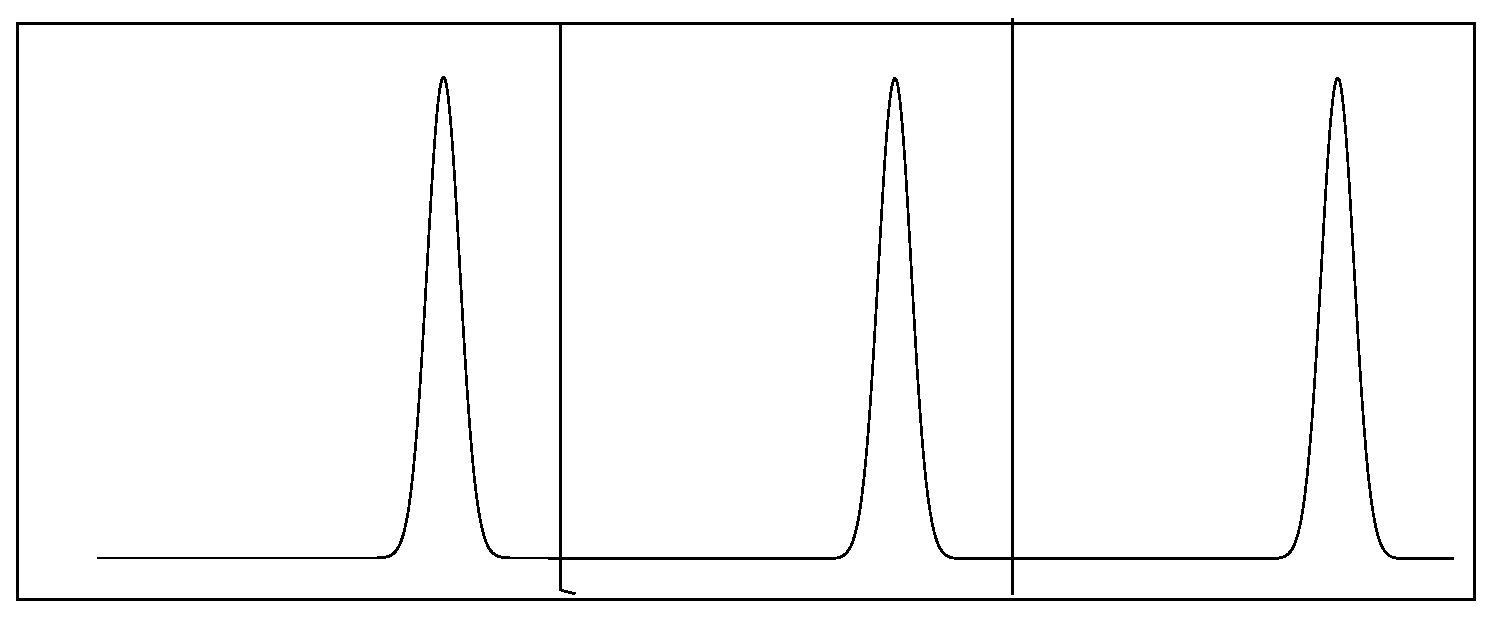
\includegraphics[width=7cm]{pulses.eps}
  \caption{Pulses}
  \label{fig:pulses}
\end{figure}
\begin{figure}[H]
  \centering
  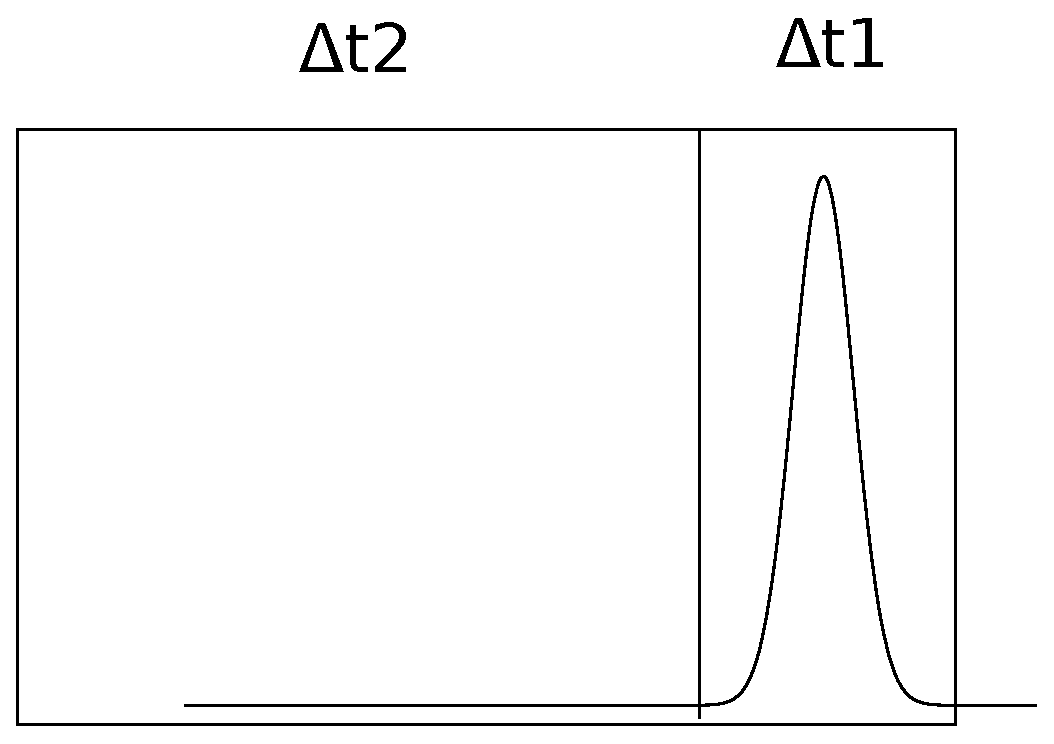
\includegraphics[width=6cm]{pulse.eps}
  \caption{Pulse}
  \label{fig:pulse}
\end{figure}
The laser pulse train can be devided in to segments as fig.\ref{fig:pulses} shows. Each segment contains two parts, one with the pulse, one with neglectable electric field, as fig.\ref{fig:pulse} shows.\\

Suppose the unraveled density matrix is $\zeta(0)$ just before the pulse. Define two matrices as follow:
\[
\zeta(\Delta t_1) = P^{\prime} \zeta(0)
\]
\[
\zeta(\Delta t_1+\Delta t_2) = P \zeta(\Delta t_{1}) = P P^{\prime} \zeta(0)
\]

Since there is no electric field in the $\Delta t_2$ period, the motion equation is $\dot{\zeta} = A \zeta$. So $\zeta(\Delta t_1+\Delta t_2) = e^{i A \Delta t_{2}} \zeta(\Delta t_{1})$.
\[
P = e^{i A \Delta t_2}
\]
\\

$P^{\prime}$ can be solve perturbatically. Define $\zeta_n (t)$ as the $n$th order solution of $\dot{\zeta} = \left( A + B E_{env}(t) \right) \zeta$ where $0< t < \Delta t_{1}$. Define $F(t)_{n} \zeta(0) = \zeta_{n}(t)$ and $G_{n}(t) \zeta(0) = \dot{\zeta_{n}(t)}$. $\frac{d F_{n}(t)}{dt} = G_{n}(t)$.\\

If the initial condition of unravel density matrix $\zeta(0)$ is known. $\zeta_{0} (t) = e^{i A t} \zeta(0)$. The next order of $\zeta$ can be obtain by:
\begin{equation}
  \label{eq:perturb}
  \zeta_{n+1}(t) = \int_0^t \left( A+B E_{env}(t) \right) \zeta_n(t)\:dt
\end{equation}
subtitute $\zeta_n(t)$ for $F_n(t)\zeta(0)$,eq.\ref{eq:perturb} becomes:
\begin{equation}
  F_{n+1}(t)\zeta(0) = \int_0^t \left( A+B E_{env}(t) \right) F_n(t)\zeta(0)\:dt
\end{equation}
remove the constant array $\zeta(0)$ which is the initial condition from both side:
\begin{equation}
  \label{eq:f}
  F_{n+1}(t) = \int_0^t \left( A+B E_{env}(t) \right) F_n(t)\:dt
\end{equation}
$F_0(t) = e^{-iAt}$ and $F_{n}(0)$ is identy matrix $I$, eq.\ref{eq:f} is independent of initial condition of $\zeta$. So $p^{\prime} = \lim_{n\rightarrow \infty}F_{n}(\Delta t_{1})$.\\

The change of unravel density matrix can be calculated with $PP^{\prime}\zeta$. After $n$ pulses the unravel density matrix become $\left( PP^{\prime} \right)^{n}\zeta$.
%\lstinputlisting[language=python,caption=plurk.py]{xxx.py}
\end{document}
